\chapter{Evaluation}
\label{ch:evaluation}
This chapter presents the evaluation of the implemented WebArgo platform through a series of experiments designed to address the research questions defined in \autoref{subsec:into:objectives:questions}. These three research questions focus on WebArgos computational capabilities when handling complex parallelizable tasks, its dynamic viability in managing fluctuating worker participation, and its ability to support heterogeneous devices as workers. Each of the following sections in this chapter corresponds to one of the research questions and presents the experimental setup, the expected outcome, and a analysis of these results.

The experiments of the evaluation utilize the implemented visualization of the Mandelbrot set, described in \autoref{sec:implementation:benchmark}, as a benchmark job. This benchmark job represents a computationally intensive test case, which can be used to demonstrate and test WebArgo's capabilities. Each task of this benchmark job covers a unique 1500x1500 area of the Mandelbrot set and all generated \ac{PNG} files have the same resolution. However, the computation time varies significantly among each of these tasks. According to the Mandelbrot function in (\ref{equ:mandelbrot}) require complex numberers that are part of the Mandelbrot set more iterations of the calculation than complex numbers that are not part of the Mandelbrot set. Therefore depends the execution time of a task on the amount of calculated points that belong to the Mandelbrot set.

Additionally, \autoref{sec:evaluation:languages} compares the performance of the various in WebArgo implemented WebAssembly environments, each supporting the execution of source code from different programming languages compiled to a WebAssembly binary.

\section{Computational Capability}
\label{sec:evaluation:computation}
\textbf{Is WebArgo capable of successfully solving large, parallelizable problems?} 
\newline
The objective of the following experiment is to evaluate WebArgo's ability to successfully execute computationally intensive, parallelizable tasks across a distributed network of volunteer workers. This empirical experiment compares the total execution time between distributed computation across multiple workers and native execution on a single computer.

\subsection{Experimental Setup}
The batch size of the benchmark job was set to 101. Therefore, only a single batch is generated and processed during all experiments and the job progress is only persisted once upon completion of all 101 tasks.

At first the benchmark job was computed on the system specified in \autoref{app:system:server} in a native Go environment using the source code of \autoref{app:code:mandelbrot3}. The resulting computation time serves as a baseline for the following experiments, because this system is later also used to host the WebArgo platform. Since this system is already required to serve WebArgo in the first place, the following experiments additionally investigate whether distributing the workload to external clients provides a performance advantage compared to utilizing the existing host system for computation. Throughout the experiments, all workers maintained available and executed only the WebArgo browser process. The benchmark job was evaluated across the following four distinct scenarios:
\begin{itemize}
    \item Two homogeneous and independent smartphones with the hardware specified in \autoref{app:system:phone} as workers, executing the client page in a Apple Safari 18.1 \cite{evaluation:safari} browser
    \item Three homogeneous and independent smartphones with the hardware specified in \autoref{app:system:phone} as workers, executing the client page in a Apple Safari 18.1 \cite{evaluation:safari} browser
    \item Three parallel Mozilla Firefox 132.0 \cite{background:firefox} browser taps of the client page on a single laptop, specified in \autoref{app:system:mymachine}
    \item Three parallel Microsoft Edge 131.0.0.0 \cite{evaluation:edge} browser taps of the client page on the same \acs{PC}, specified in \autoref{app:system:mypc}
\end{itemize}

\subsection{Expectations}
It is expected that all tasks of the benchmark job will be scheduled as intended and distributed over all participating workers and each task result is successfully received by the server and saved on the server. To verify if this process was successful, each worker is monitored through the interface of the client page during the experiment and after the experiment is the implemented mandelbrot page (\autoref{sec:implementation:benchmark}) utilized to examine the generated task results.

Additinally, all experiments are carried out using the interactive dashboard page (\autoref{subsec:implementation:dashboard-page}) to start and monitor the execution of the benchmark job. It is expected that all features of this application work as intended and the job progress as well as all participating workers can be monitored in real-time.

(TODO) Change calculation from latency to overhead = latency + file Size input \& wasm + gluecode (?) + (latency) + file size result

Furthermore, based on the theoretical model presented in \autoref{sec:background:theory}, distributing the benchmark job across multiple workers should reduce the total execution time of a job when the number of workers $N$ exceeds the threshold value represented in the inequality term of \eqref{equ:transformation2}. To estimate this threshold value of $N$ for all previously listed experiment scenarios the amount of tasks $T$ was set to 101 and an internet latency of 32 ms \cite{backend:latency} was assumed for $t_{L}$. Since the computation times $t_{Native}$ and $t_{Virtual}$ are not equal for all 101 tasks, a computationally intensive task - handling the center of the Mandelbrot set - was selected to represent these computation times. This single task has been executed and measured independently on the native Go environment on the server system as well as on the WebAssembly browser environment through the WebArgo platform for each device participating in the experiment as worker. The computation time $t_{Native}$ of this computationally intensive task was measured to be 34.60 seconds on the server system specified in \autoref{app:system:server}. The corresponding computation time $t_{Virtual}$ of the same task was measured to be 52.56 seconds using the Apple Safari 18.1 \cite{evaluation:safari} browser on a smartphone specified in \autoref{app:system:phone}, 1 minute and 34.8 seconds using the Mozilla Firefox 132.0 \cite{background:firefox} browser on the laptop specified in \autoref{app:system:mymachine} and 1 minute and 28.2 seconds using the Microsoft Edge 131.0.0.0 \cite{evaluation:edge} browser on the \acs{PC} specified in \autoref{app:system:mypc} With this information the amount of workers $N$ - expected to provide a performance advantage compared to the native code execution - was calculated with the inequality term of \eqref{equ:transformation2} for each scenario:
\begin{itemize}
    \item \textbf{Smartphones:} $N > 1.5$, meaning two or more smartphones are expected to achieve a performance improvement 
    \item \textbf{Laptops:} $N > 2.8$, meaning three or more laptops are expected to achieve a performance improvement
    \item \textbf{PCs:} $N > 2.6$, meaning three or more \acs{PC}s are expected to achieve a performance improvement
\end{itemize}

\subsection{Results}
The benchmark job was successfully computed in every experiment and all features of the web application behaved as intended. \autoref{fig:evaluation:experiment-A} compares the measured execution times of the different experiments to the baseline time of the server.

The native execution on the server system completed all 101 tasks in an average execution time $t_{ExSeq}$ of 10 minutes and 45 seconds across three runs. Distributing the benchmark job across the two smartphone workers resulted in a total execution time $t_{ExDist}$ of 10 minutes and 12 seconds, and therefore faster than the baseline as predicted. With three smartphone workers, the execution time further decreased to 6 minutes and 39 seconds, representing a performance improvement of 38\% compared to the native execution on the server.

Distributing the benchmark job across three browser taps on the laptop took 12 minutes and 56.4 seconds to complete the total workload. This approach did not achieve a performance improvement compared to the native code execution on the server. However, distributing the benchmark job across three browser taps on the \acs{PC} complete the total workload in only 9 minutes and 52.8 seconds and therefore faster than the baseline of the server. These two experiments show that a single device can be successfully utilized to participate in WebArgo with running multiple worker processes in parallel, and therefore effectively allows to expand the job progress computed by a single device. But it can not be expected that a single browser tab in this scenario will behave in the same way as an independent device. The behavior of multiple worker tabs on a single device most likely depends on the devices hardware, the amount of available \acs{CPU} cores and the browser and operating system used.
\begin{figure}[htbp]
    \centering
    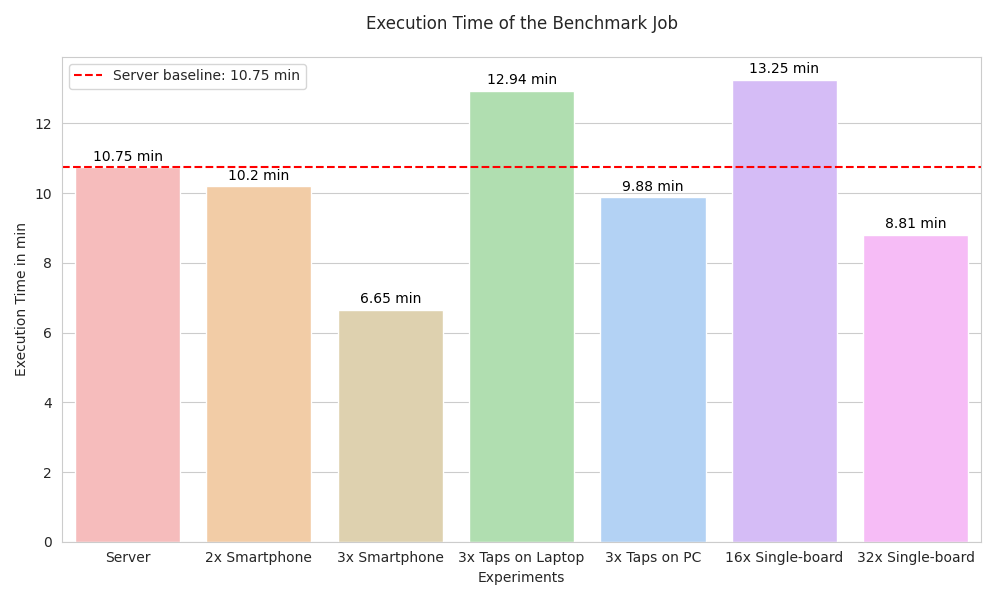
\includegraphics[width=0.95\textwidth]{gfx/figures/Evaluation_A.png}
    \caption{WebArgo Execution Time Compared to Native Execution Time}
    \label{fig:evaluation:experiment-A}
\end{figure}
~\\
(TODO) Add amduhls law speedup caalculation

These results validate the predictions of the theoretical model presented in \autoref{sec:background:theory}. Using the calculation of the inequality term in \eqref{equ:transformation2} allowed to predict that two or more smartphone workers would achieve a faster execution time compared to the native baseline, which was confirmed by the experiment. This improvement further scaled with three smartphone workers, reducing the execution time by a total of 38\% compared to the server baseline.

The experiments with parallel worker browser tabs on single devices revealed, that a single worker is able to enhance its computational participation by executing multiple worker instances simultaneously. However, the measured performance difference between the laptop and \acs{PC} is suggesting, that the execution of multiple worker instances is limited by the devices hardware.

Furthermore, these experimental results support the theoretical assumption from \autoref{sec:background:theory} that the performance gain through distributed computation on multiple workers is able to outweigh the additional overhead of communicating through the internet and the longer computation time $t_{Virtual}$ in the WebAssembly environment. This validates that even with these performance constraints, WebArgo can effectively leverage parallel processing through volunteer computing to reduce the total computation time of a job. The achieved performance improvement scales with the number of participating workers $N$.

\section{Dynamic Viability}
\label{sec:evaluation:dynamic}
\textbf{Is the WebArgo platform stable in a environment with dynamic clients?}
\newline
The second research question investigates whether WebArgo maintains stability in an environment with dynamic clients, addressing a fundamental challenge in volunteer computing where worker participation is inherently unpredictable and therefore dynamic. This evaluation is crucial, as a key feature of WebArgo is to maintain operational despite workers joining or leaving at any time. Hence, the following experiments in this section evaluate WebArgo's ability to handle fluctuating worker participation.

\subsection{Experimental Setup}
To evaluate WebArgo's dynamic viability, the platform was tested in a controlled environment with manually connecting or disconnecting workers. The experiments utilized 32 single-board computers specified in \autoref{app:system:pi}, each running a headless Mozilla Firefox 133.0 \cite{background:firefox2} browser to participate in WebArgo as a worker through the cleint web application. Again, the Mandelbrot benchmark job was utilized for these experiments. All single-board computers used in this experiment are part of the \emph{Pi-lab} from h\_da, providing a practical infrastructure to interact with multiple Raspberry Pi computers. The task timeout to enable rescheduling of aborted tasks was set to be 60 seconds throughout the benchmark job. The following two experiments were conducted to simulate a dynamic environment where workers join or leave the network during the execution of an active job:
\begin{enumerate}
    \item Disconnecting of 8 workers (25\% of all conneted workers) after about 50\% of total job completion 
    \item Starting with 8 connected workers and gradually connecting more devices until 32 workers are connected
\end{enumerate}
Additionally, an experiment with all 32 single-board computers computing the benchmark job while maintaining a stable connection to the platform was performed. The total execution time of this experiment is used as a baseline time to compare the results of the previous experiments.

\subsection{Expectations}
It is expected that all 101 tasks of the bechmark job are successfully completed, regardless of the fluctuating behaviour of workers. Hence, aborted task from disconnected workers are expected to be rescheduled to other availabile workers, and workers wich are connecting while the active job is already running are expected to automatically setup the corresponding WebAssembly environment and then immediately participate as workers.

However, it is expected that the total execution time of both experiments will be longer than the baseline time, since in these scenarios less worker instances are consistently participating throughout the computation of the job. 

\subsection{Results}
The benchmark job was successfully computed in both experiments and all connecting workers have actively participated in computing the workload of the job. Therefore, these experimental results demonstrate WebArgo's robust handling of dynamic worker participation. \autoref{fig:evaluation:experiment-B} displays the total computaion time of both experiments compared to the basline computation time of 32 permanently connected single-board computers as workers.

\begin{figure}[htbp]
    \centering
    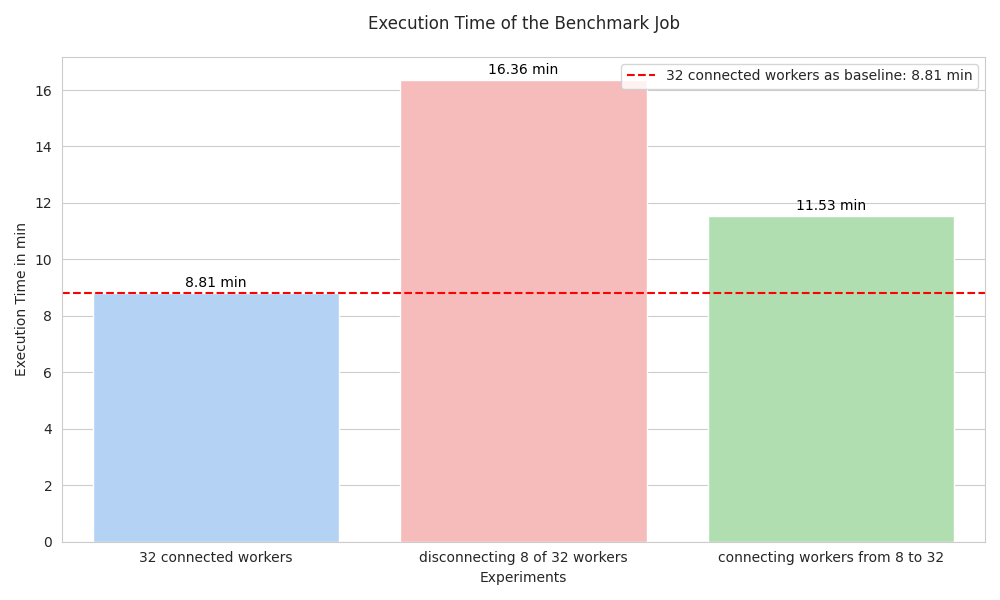
\includegraphics[width=0.95\textwidth]{gfx/figures/Evaluation_B.png}
    \caption{WebArgo Execution Time in Dynamic Environment}
    \label{fig:evaluation:experiment-B}
\end{figure}
~\\
In experiment 1, the WebArgo platform successfully demonstrated reliable task redistribution when workers are disconnecting during the computation of a task. The implemented timeout mechanism effectively rescheduled all 8 aborted tasks distributed to the 8 manually disconnected workers. The system maintained consistent progress despite losing up 25\% of the initial worker pool, though with a expected increases of the total computation time to 16 minutes and 21.6 seconds.

During experiment 2, the WebArgo platform successfully integrated new workers as they joined, with each additional worker immediately receiving and computing tasks from the current batch after they successful initialized the corresponding WebAssembly environment. Since this experiment started with only 25\% of the amount of workers compared to the baseline experiment, it was expected that the total computation time is slower than the baseline. Corresponding, the total execution time of this experiment was 11 minutes and 31.8 seconds. 
\\~\\
Both experiments demonstrated that the WebArgo platform can maintain operation continuity despite significant worker pool fluctuations. This validates WebArgo's implementation for dynamic worker participation and confirms, that it is suitability for real-world volunteer computing scenarios where the availability of a worker device is not guaranteed.

\section{Heterogeneous Viability}
\label{sec:evaluation:heterogen}
\textbf{Does WebArgo support a diverse range of client devices without issues?}
The third research question examines WebArgo's capability to effectively support diverse client devices as workers, therefore also addressing a critical requirement for volunteer computing platforms. As the pool of potential worker devices in a real-world environment is expected to be diverse in hardware, software and operating systems \cite{intro:diverseDevices}, the following experiment is used to evaluate whether WebArgo can successfully operate with a heterogeneous group of participating workers.

\subsection{Experimental Setup}
To evaluate the platform's support for heterogeneous devices, a diverse set of everyday consumer devices was assembled to participate simultaneously in the benchmark job through the WebArgo platform. The following four devices represent different hardware architectures, various operating systems (iOS, Windows, and Ubuntu), and also different browser environments (Apple Safari 18.1 \cite{evaluation:safari}, Mozilla Firefox 132.0 \cite{background:firefox}, and Microsoft Edge 131.0.0.0 \cite{evaluation:edge}):
\begin{itemize}
    \item One smartphone as specified in \autoref{app:system:phone}
    \item One laptop as specified in \autoref{app:system:mymachine}, executing 3 worker tabs in parallel
    \item One \acs{PC} as specified in \autoref{app:system:mypc}, executing 3 worker tabs in parallel
    \item One tablet as specified in \autoref{app:system:tablet}
\end{itemize}
All of these devices where found in one hoeshold to demonstrate the easy accessibility to a potential performance improvement of a computational intensive job by leveraging the WebArgo platform.

\subsection{Expectations}
It is expected that the bechmark job is successfully computed and that all participating workers are able to compute their scheduled tasks, regardless of the heterogeneous pool of connected devices. Furthermore, this set of devices - representing a single household - is expected to achieve a significant performance improvement compared to the baseline execution time of the natively computed Mandelbrot visualization on the server.  

\subsection{Results}
(TODO) Amduhls law speedup

The Mandelbrot visualization job was again successfully computed and all participating workers were able to compute the tasks that have been distributed to them. Therefore, this experiment demonstrated WebArgo's support for heterogeneous devices as workers. All devices successfully connected to the platform, initialized their WebAssembly environments, and computed their assigned tasks without any occuring issues. The WebSocket connections remained stable and the WebWorker-WebAssembly environment was effortlessly established across all corresponding browsers, each being preinstalled on the devices by default. \autoref{fig:evaluation:experiment-C} displays the total execution time of this experiment compared to the basline execution time of the native server environment measured in \autoref{sec:evaluation:computation}.
\begin{figure}[htbp]
    \centering
    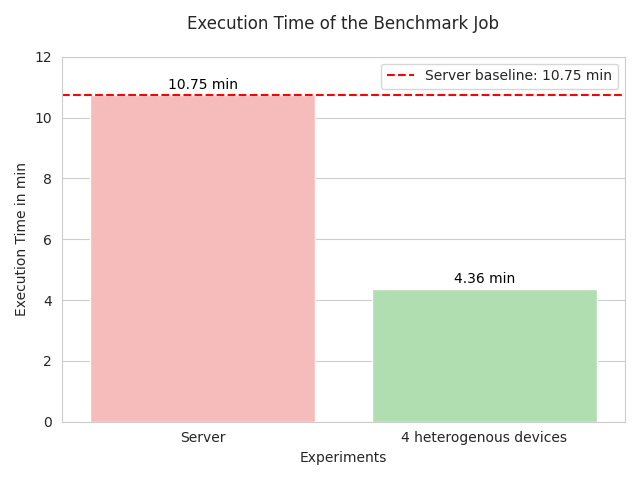
\includegraphics[width=0.95\textwidth]{gfx/figures/Evaluation_C.png}
    \caption{WebArgo Execution Time with Heterogeneous Set of Workers}
    \label{fig:evaluation:experiment-C}
\end{figure}
~\\
Using the setup of this experiment, the benchmark job was already completed after 4 minutes and 21.6 seconds. This represents a performance improvement of 59\% compared to the native execution on the server. The substantial reduction in execution time demonstrates the effectiveness of WebArgo's approach to volunteer computing, even when considering the additional overhead of network communication, task scheduling and computation time $t_{Virtual}$ in a WebAssembly environment. This validates that WebArgo can effectively utilize an environment of heterogeneous devices to achieve significant performance improvements compared to native code execution on a  single system.
\\~\\
The implemented web interface of the client page adapted appropriately to all different screen sizes and resolutions, providing a consistent user experience across all devices. Additionally, the WebWorker implementation effectively prevented any freezing effects of the browser \ac{UI} during the computation of tasks for all participating workers. Therefore, the web application maintained responsiv throughout the experiment and provided real-time monitoring of each worker, as intended.
\\~\\
These results validate that WebArgo successfully leveraged WebAssembly's platform independence to enable consistent computation across different architectures, while the web-based approach provided a uniform and easy-to-use application, accessible on any device with a modern browser. This confirms that WebArgo achieves its intended design goal.

\section{Comparison of Implemented WebAssembly Environments}
\label{sec:evaluation:languages}
As WebArgo currently supports three different programming languages as source for jobs, this section compares the performance of these implemented WebAssembly environments. Each of these programming languages utilizes a unique compilation toolchain to generate the executable WebAssembly binary files and unique JavaScript glue code to handel the corresponding WebAssembly binary in a browser environment, as described in \autoref{sec:methodology:wasm}. A comparison of these implementations can provide valuable insights for potential administrators, which develop new jobs served by a hostet WebArgo platform.

\subsection{Prime Numbers}
The three implemented WebAssembly environments were evaluated with three other benchmark jobs, each implemented in either C++, Go or Python. Each of these benchmark jobs finds and lists all prime numbers in the range from $0$ to $10.000.000$ and is divided in 10 distinct tasks, each processing a unique intervall of 1 million numbers. All of these 3 prime number jobs have been executed through the WebArgo platform by a single worker instance, executed in a Apple Safari 18.1 \cite{evaluation:safari} browser on the smartphone specified in \autoref{app:system:phone}.
\\~\\
\autoref{fig:evaluation:experiment-D} compares the total execution time of each prime number job executed in this experiment, revealing significant variations in performance across the different environments. The C++ WebAssembly environment, leveraging the toolchain of emscripten \cite{methodology:emcc}, demonstrated the best computational performance and successfully completed all 10 tasks in only 5.9 seconds. The Go WebAssembly environment, compiled and initialized with the tools provided by Go \cite{methodology:go}, achieved similar but slower execution time of 7.2 seconds for the prime number job. In contrast to these results, the Python WebAssembly environment, utilizing the Pyodide library \cite{methodology:pyodie}, took a total of 156.6 seconds to compute the same workload.
\begin{figure}[htbp]
    \centering
    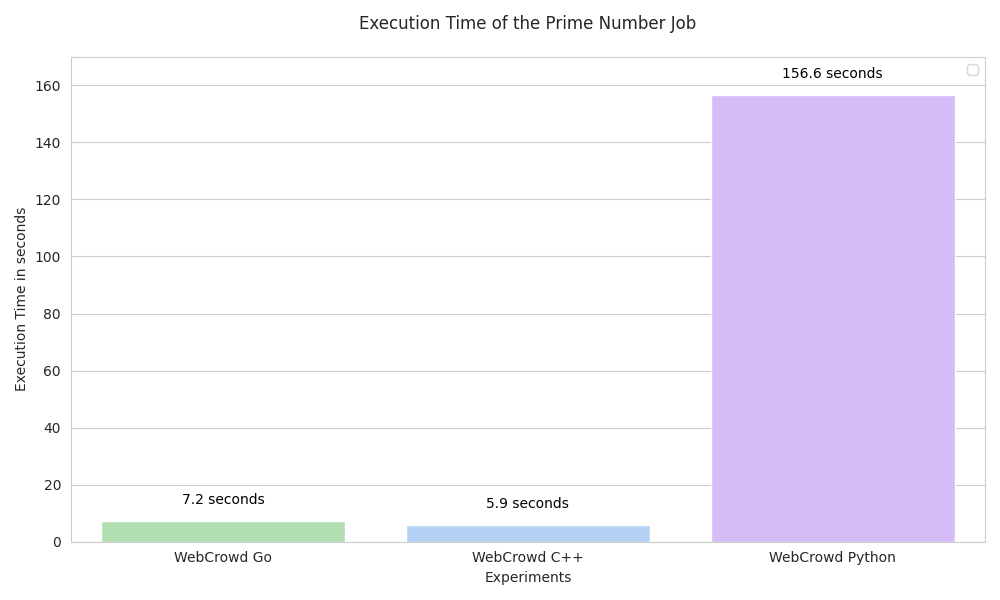
\includegraphics[width=0.95\textwidth]{gfx/figures/Evaluation_D.png}
    \caption{WebArgo Execution Time of Different WebAssembly Environments}
    \label{fig:evaluation:experiment-D}
\end{figure}
~\\
Despite the fact that all three jobs executed the same workload with a WebAssembly binary on the same system and in the same browser, the execution time of each job varied significantly. The emscripten \cite{methodology:emcc} WebAssembly toolchain demonstrated the best computational performance in this scenario, however it has not been further investigated why this is the case.

\subsection{Mandelbrot Set}
Additionally to the previous experiment, the implemented C++ and Go WebAssembly environments are further compared in this section. Both environments have demonstrated a similar performance when computing the prime number job. However, the following experiments again utilize the visualization of the Mandelbrot set described in \autoref{sec:implementation:benchmark}. The Go source code, compiled with Go \cite{methodology:go} to WebAssembly, can be found in \autoref{app:code:mandelbrot2}, and the according C++ source code, compiled by the emscripten \cite{methodology:emcc} toolchain, can be found in \autoref{app:code:mandelbrot4}.

To compare the performance of both environments, first a single computationally intensive task, generating the center of the Mandelbrot set, was computed in each WebArgo environment by a worker instance executed in a Apple Safari 18.1 \cite{evaluation:safari} browser on the smartphone specified in \autoref{app:system:phone}. Then, the same worker instance was used to compute all 101 tasks of the Go Mandelbrot benchmark job and the C++ Mandelbrot benchmark job. Additionally, all of these experiments were repeated with corresponding native environments on the server, specified in \autoref{app:system:server}.

\autoref{fig:evaluation:experiment-E} compares the measured total execution time of this experiment compared to the basline execution time on the native server environment. The C++ WebAssembly environment was able to compute the computationally havy task in only 46.6 seconds and was therefore again faster than the corresponding Go WebAssembly environment, which took 52.56 seconds to compute the same workload. This represents a performance advantage of 11\% for the C++/emscripten approach compared to the Go toolchain, graphically displayed in \autoref{fig:evaluation:experiment-E1} on the right side. This performance advantage increased to 20\% when processing the entire benchmark job, as displayed in \autoref{fig:evaluation:experiment-E2}.
\begin{figure}[htbp]
    \myfloatalign
    \subfloat[Single Computationally Intensive Task]{
        \label{fig:evaluation:experiment-E1}
        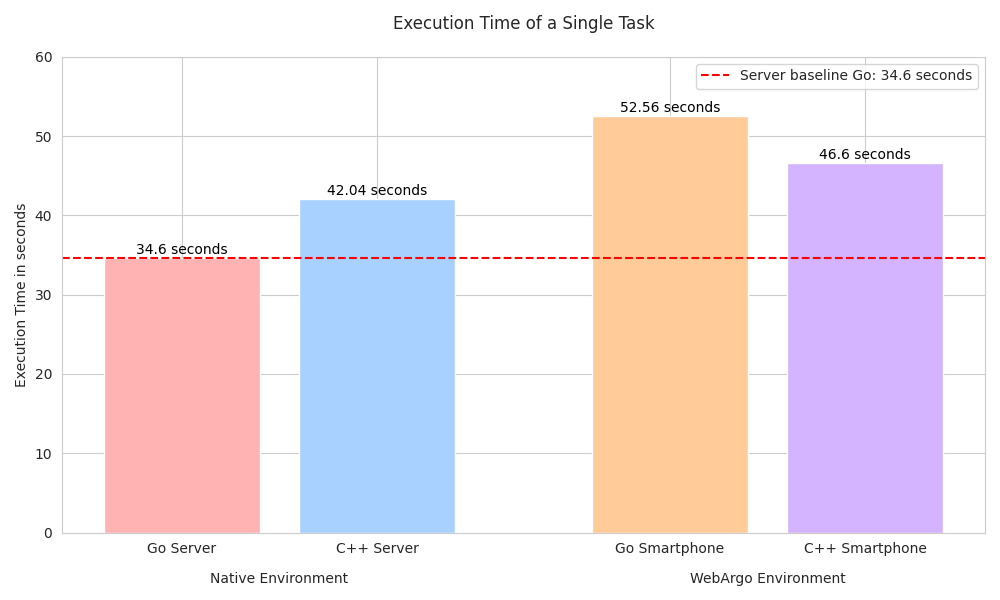
\includegraphics[width=0.95\textwidth]{gfx/figures/Evaluation_E-1.png}
    } \\
    \subfloat[Mandelbrot Benchmark Job]{
        \label{fig:evaluation:experiment-E2}
        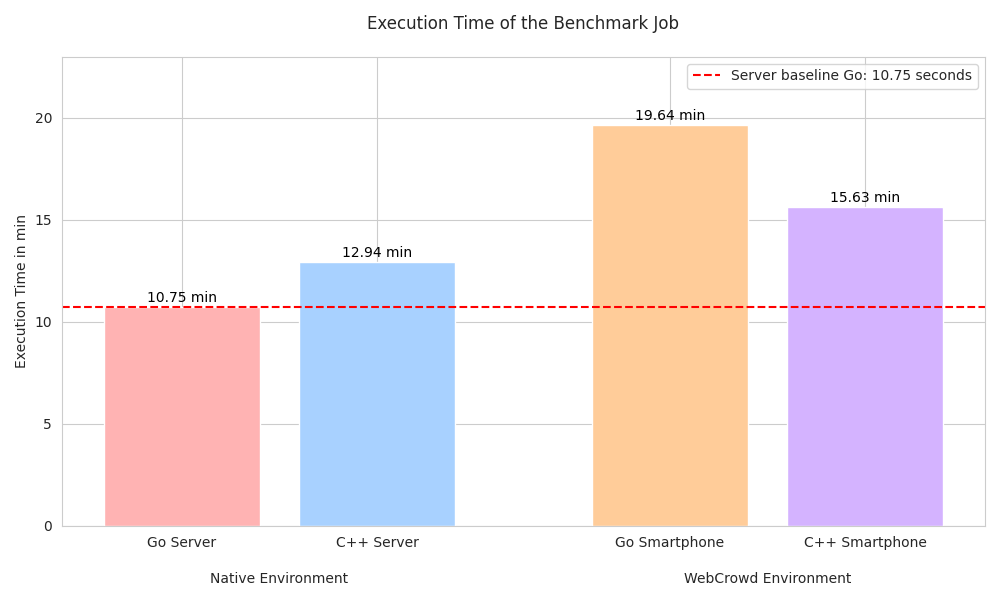
\includegraphics[width=.95\linewidth]{gfx/figures/Evaluation_E-2.png}
    }
    \caption{Comparison of C++ and Go Execution Time}
    \label{fig:evaluation:experiment-E}
\end{figure}
~\\
This investigation confirms the performance advantage of the implemented C++ WebAssembly environment over the implemented Go WebAssembly environment.